\documentclass[14pt]{extbook}
\usepackage{multicol, enumerate, enumitem, hyperref, color, soul, setspace, parskip, fancyhdr} %General Packages
\usepackage{amssymb, amsthm, amsmath, bbm, latexsym, units, mathtools} %Math Packages
\everymath{\displaystyle} %All math in Display Style
% Packages with additional options
\usepackage[headsep=0.5cm,headheight=12pt, left=1 in,right= 1 in,top= 1 in,bottom= 1 in]{geometry}
\usepackage[usenames,dvipsnames]{xcolor}
\usepackage{dashrule}  % Package to use the command below to create lines between items
\newcommand{\litem}[1]{\item#1\hspace*{-1cm}\rule{\textwidth}{0.4pt}}
\pagestyle{fancy}
\lhead{Progress Quiz 10}
\chead{}
\rhead{Version C}
\lfoot{6232-9639}
\cfoot{}
\rfoot{Fall 2020}
\begin{document}

\begin{enumerate}
\litem{
Describe the end behavior of the polynomial below.\[ f(x) = 9(x - 8)^{3}(x + 8)^{4}(x - 3)^{5}(x + 3)^{7} \]\begin{enumerate}[label=\Alph*.]
\begin{multicols}{2}\item 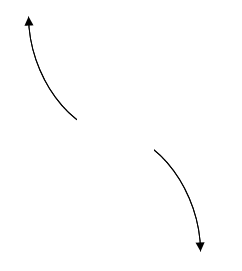
\includegraphics[width = 0.3\textwidth]{../Figures/polyEndBehaviorAC.png}\item 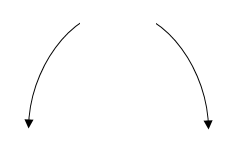
\includegraphics[width = 0.3\textwidth]{../Figures/polyEndBehaviorBC.png}\item 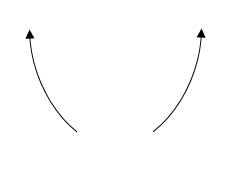
\includegraphics[width = 0.3\textwidth]{../Figures/polyEndBehaviorCC.png}\item 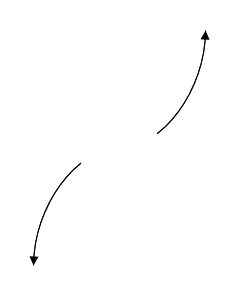
\includegraphics[width = 0.3\textwidth]{../Figures/polyEndBehaviorDC.png}\end{multicols}\item None of the above.
\end{enumerate} }
\litem{
Construct the lowest-degree polynomial given the zeros below. Then, choose the intervals that contain the coefficients of the polynomial in the form $x^3+bx^2+cx+d$.\[ -2 + 3 i \text{ and } 2 \]\begin{enumerate}[label=\Alph*.]
\item \( b \in [0.54, 1.25], c \in [-9, -2], \text{ and } d \in [1, 8] \)
\item \( b \in [0.54, 1.25], c \in [-2, 1], \text{ and } d \in [-4, 0] \)
\item \( b \in [1.7, 2.1], c \in [4, 7], \text{ and } d \in [-29, -22] \)
\item \( b \in [-2.25, -0.75], c \in [4, 7], \text{ and } d \in [25, 29] \)
\item \( \text{None of the above.} \)

\end{enumerate} }
\litem{
Describe the zero behavior of the zero $x = 2$ of the polynomial below.\[ f(x) = -8(x - 2)^{9}(x + 2)^{12}(x + 6)^{7}(x - 6)^{9} \]\begin{enumerate}[label=\Alph*.]
\begin{multicols}{2}\item 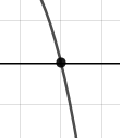
\includegraphics[width = 0.3\textwidth]{../Figures/polyZeroBehaviorCopyAC.png}\item 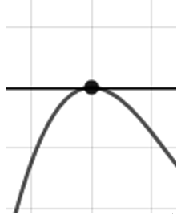
\includegraphics[width = 0.3\textwidth]{../Figures/polyZeroBehaviorCopyBC.png}\item 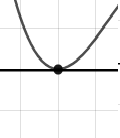
\includegraphics[width = 0.3\textwidth]{../Figures/polyZeroBehaviorCopyCC.png}\item 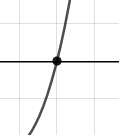
\includegraphics[width = 0.3\textwidth]{../Figures/polyZeroBehaviorCopyDC.png}\end{multicols}\item None of the above.
\end{enumerate} }
\litem{
Construct the lowest-degree polynomial given the zeros below. Then, choose the intervals that contain the coefficients of the polynomial in the form $ax^3+bx^2+cx+d$.\[ \frac{6}{5}, \frac{-1}{3}, \text{ and } \frac{2}{5} \]\begin{enumerate}[label=\Alph*.]
\item \( a \in [70, 82], b \in [34, 42], c \in [-60, -51], \text{ and } d \in [10, 14] \)
\item \( a \in [70, 82], b \in [-103, -90], c \in [-5, -2], \text{ and } d \in [10, 14] \)
\item \( a \in [70, 82], b \in [91, 96], c \in [-5, -2], \text{ and } d \in [-15, -9] \)
\item \( a \in [70, 82], b \in [-103, -90], c \in [-5, -2], \text{ and } d \in [-15, -9] \)
\item \( a \in [70, 82], b \in [78, 91], c \in [-17, -13], \text{ and } d \in [-15, -9] \)

\end{enumerate} }
\litem{
Which of the following equations \textit{could} be of the graph presented below?
\begin{center}
    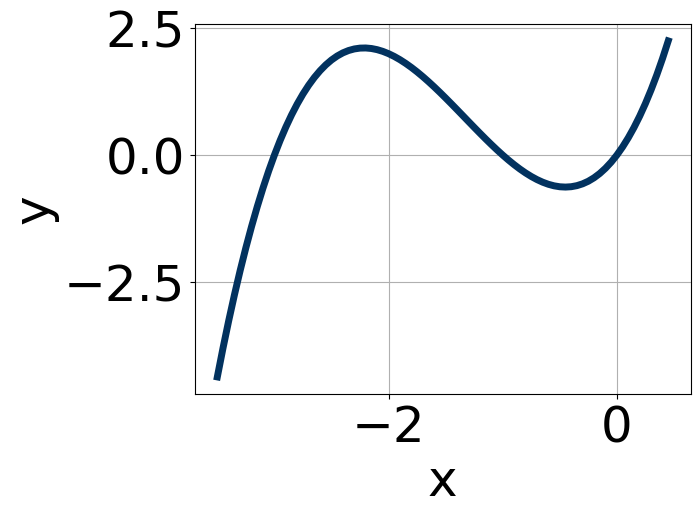
\includegraphics[width=0.5\textwidth]{../Figures/polyGraphToFunctionC.png}
\end{center}
\begin{enumerate}[label=\Alph*.]
\item \( 15x^{5} (x + 3)^{5} (x + 1)^{5} \)
\item \( 11x^{9} (x + 3)^{4} (x + 1)^{9} \)
\item \( 12x^{7} (x + 3)^{4} (x + 1)^{6} \)
\item \( -19x^{5} (x + 3)^{10} (x + 1)^{9} \)
\item \( -9x^{7} (x + 3)^{11} (x + 1)^{7} \)

\end{enumerate} }
\litem{
Describe the zero behavior of the zero $x = -4$ of the polynomial below.\[ f(x) = 4(x + 4)^{8}(x - 4)^{13}(x + 9)^{7}(x - 9)^{8} \]\begin{enumerate}[label=\Alph*.]
\begin{multicols}{2}\item 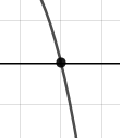
\includegraphics[width = 0.3\textwidth]{../Figures/polyZeroBehaviorAC.png}\item 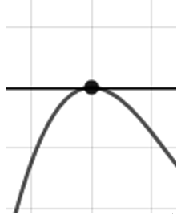
\includegraphics[width = 0.3\textwidth]{../Figures/polyZeroBehaviorBC.png}\item 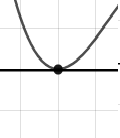
\includegraphics[width = 0.3\textwidth]{../Figures/polyZeroBehaviorCC.png}\item 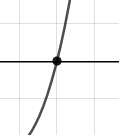
\includegraphics[width = 0.3\textwidth]{../Figures/polyZeroBehaviorDC.png}\end{multicols}\item None of the above.
\end{enumerate} }
\litem{
Describe the end behavior of the polynomial below.\[ f(x) = -7(x + 2)^{4}(x - 2)^{7}(x + 9)^{4}(x - 9)^{6} \]\begin{enumerate}[label=\Alph*.]
\begin{multicols}{2}\item 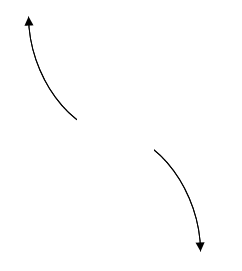
\includegraphics[width = 0.3\textwidth]{../Figures/polyEndBehaviorCopyAC.png}\item 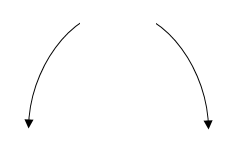
\includegraphics[width = 0.3\textwidth]{../Figures/polyEndBehaviorCopyBC.png}\item 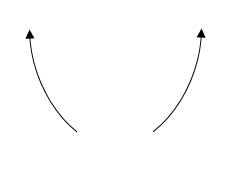
\includegraphics[width = 0.3\textwidth]{../Figures/polyEndBehaviorCopyCC.png}\item 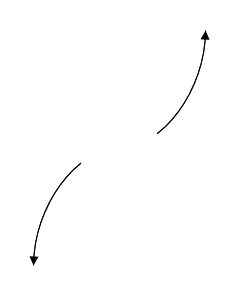
\includegraphics[width = 0.3\textwidth]{../Figures/polyEndBehaviorCopyDC.png}\end{multicols}\item None of the above.
\end{enumerate} }
\litem{
Construct the lowest-degree polynomial given the zeros below. Then, choose the intervals that contain the coefficients of the polynomial in the form $x^3+bx^2+cx+d$.\[ 3 + 5 i \text{ and } -3 \]\begin{enumerate}[label=\Alph*.]
\item \( b \in [2.51, 4.34], c \in [15.82, 16.89], \text{ and } d \in [-103.2, -101.1] \)
\item \( b \in [-1.5, 2.17], c \in [-1.04, 0.81], \text{ and } d \in [-9.6, -7.5] \)
\item \( b \in [-4.81, -1.83], c \in [15.82, 16.89], \text{ and } d \in [99.1, 105] \)
\item \( b \in [-1.5, 2.17], c \in [-2.18, -1.34], \text{ and } d \in [-19.2, -13.9] \)
\item \( \text{None of the above.} \)

\end{enumerate} }
\litem{
Which of the following equations \textit{could} be of the graph presented below?
\begin{center}
    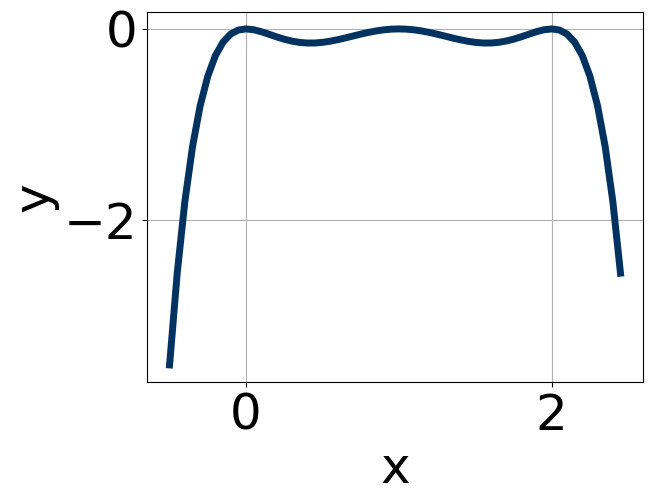
\includegraphics[width=0.5\textwidth]{../Figures/polyGraphToFunctionCopyC.png}
\end{center}
\begin{enumerate}[label=\Alph*.]
\item \( -17x^{6} (x - 2)^{8} (x - 1)^{4} \)
\item \( -16x^{8} (x - 2)^{4} (x - 1)^{11} \)
\item \( 13x^{8} (x - 2)^{8} (x - 1)^{11} \)
\item \( 18x^{8} (x - 2)^{6} (x - 1)^{4} \)
\item \( -2x^{8} (x - 2)^{5} (x - 1)^{7} \)

\end{enumerate} }
\litem{
Construct the lowest-degree polynomial given the zeros below. Then, choose the intervals that contain the coefficients of the polynomial in the form $ax^3+bx^2+cx+d$.\[ -4, \frac{3}{5}, \text{ and } \frac{5}{3} \]\begin{enumerate}[label=\Alph*.]
\item \( a \in [14, 16], b \in [-94, -92], c \in [149, 155], \text{ and } d \in [-66, -56] \)
\item \( a \in [14, 16], b \in [20, 30], c \in [-121, -118], \text{ and } d \in [53, 62] \)
\item \( a \in [14, 16], b \in [20, 30], c \in [-121, -118], \text{ and } d \in [-66, -56] \)
\item \( a \in [14, 16], b \in [-83, -73], c \in [46, 50], \text{ and } d \in [53, 62] \)
\item \( a \in [14, 16], b \in [-29, -22], c \in [-121, -118], \text{ and } d \in [-66, -56] \)

\end{enumerate} }
\end{enumerate}

\end{document}